\section{Results and Analysis}

\subsection{Methodology and Experimental Setup}
All results were obtained on an NVIDIA GeForce GTX 1080 Ti (11GB GDDR5X) paired with an Intel Core i7-8700K CPU @ 4.8 GHz and 32GB DDR4 RAM, running Ubuntu 24.04.3 LTS. The test dataset consists of a dense point cloud scan of an urban environment containing 648,433 points.

To ensure robust results, the voxelizers were evaluated across a wide parameter space:
\begin{itemize}
    \item \textbf{Voxel Sizes:} 0.25, 0.5, 0.75, 1.0, 1.25.
    \item \textbf{Block Sizes:} 1, 2, 4, 8, 16, 32, 64, 256, 512, 1024 threads per block.
    \item \textbf{Hash-Table Capacity Factors:} 2, 3, and 4 times the input point count.
\end{itemize}
Every configuration was executed 100 times to obtain average execution times and minimize transient system load variations.

\subsection{Overall Performance: CPU vs. GPU}
The transition to GPU-based voxelization yields substantial performance improvements. As shown in Tables \ref{tab:cpu_min} and \ref{tab:cpu_max}, the GPU implementations achieve speedup factors ranging from \textbf{9.5$\times$ to 15.5$\times$} compared to the CPU.

The most significant gains occur at smaller voxel sizes (e.g., 0.25), where the massive parallelism of the GPU is fully exploited. Even in worst-case GPU scenarios, the speedup remains between 6.1$\times$ and 12.2$\times$.

\begin{table}[H]
\centering
\begin{tabular}{|c|c|c|c|c|c|}
\hline
\textbf{Voxel Size} & \textbf{CPU (ms)} & \textbf{Morton (ms)} & \textbf{Hash CF2 (ms)} & \textbf{Hash CF3 (ms)} & \textbf{Hash CF4 (ms)} \\
\hline
0.25 & 429.09 & 36.61 & 27.70 & 29.57 & 29.10 \\
0.5 & 335.89 & 29.14 & 26.20 & 28.30 & 28.57 \\
0.75 & 272.39 & 27.11 & 25.89 & 26.57 & 27.74 \\
1.0 & 253.67 & 25.71 & 25.67 & 26.99 & 27.46 \\
1.25 & 240.00 & 25.18 & 25.85 & 27.24 & 28.28 \\
\hline
\end{tabular}
\caption{CPU vs Minimum GPU Voxelization Time}
\label{tab:cpu_min}
\end{table}

\begin{table}[H]
\centering
\begin{tabular}{|c|c|c|c|c|c|}
\hline
\textbf{Voxel Size} & \textbf{CPU (ms)} & \textbf{Morton (ms)} & \textbf{Hash CF2 (ms)} & \textbf{Hash CF3 (ms)} & \textbf{Hash CF4 (ms)} \\
\hline
0.25 & 429.09 & 40.46 & 35.25 & 37.48 & 41.82 \\
0.5 & 335.89 & 31.18 & 33.87 & 35.53 & 40.00 \\
0.75 & 272.39 & 28.62 & 33.80 & 36.09 & 39.12 \\
1.0 & 253.67 & 27.63 & 33.36 & 35.26 & 38.53 \\
1.25 & 240.00 & 28.64 & 34.41 & 36.85 & 39.06 \\
\hline
\end{tabular}
\caption{CPU vs Maximum GPU Voxelization Time}
\label{tab:cpu_max}
\end{table}

\subsection{Detailed Analysis of GPU Methods}

\subsubsection{Morton-Code Voxelizer}
The Morton-based approach demonstrates consistent and predictable performance. It excels at larger voxel sizes (1.25 and above) where spatial coherence is high.
\begin{itemize}
    \item \textbf{Timing Breakdown:} The runtime is dominated by the \textbf{sorting stage} (0.90--1.02\,ms), which is constant across tests. Point accumulation takes 0.24--1.08\,ms.
    \item \textbf{Sensitivity:} Very small block sizes (1--4 threads) significantly slow down Morton-code generation (up to 1.07\,ms), whereas larger blocks stabilize this step to $\approx$0.04\,ms.
\end{itemize}

\subsubsection{Hash-Table Voxelizer}
The hash-based method is generally faster for small-to-medium voxel sizes but is highly sensitive to the \textbf{Capacity Factor (CF)}.
\begin{itemize}
    \item \textbf{CF 2 (Highest Efficiency):} Offers the best performance (25.67\,ms at voxel size 1.0) due to low memory overhead and fast device-to-host transfers ($\approx$2.71\,ms).
    \item \textbf{CF 3 \& 4 (Higher Overhead):} Increasing the table size reduces collisions but incurs significant penalties in initialization and memory transfer. CF 4 is 5--10\,ms slower than CF 2, with transfer times rising to 5.26\,ms.
\end{itemize}

\subsection{Parameter Sensitivity and Bottlenecks}

\subsubsection{Impact of Voxel Size}
Smaller voxel sizes generate a larger number of unique entries. This favors the \textbf{Hash-Table (CF 2)} method, which handles high fragmentation efficiently. Conversely, larger voxel sizes favor the \textbf{Morton} method, which benefits from predictable memory access patterns when spatial data is less fragmented.

\subsubsection{Impact of Block Size}
Both methods exhibit similar responses to thread block sizing:
\begin{itemize}
    \item \textbf{1--4 threads (Inefficient):} Severe performance penalties due to insufficient warp utilization.
    \item \textbf{8--256 threads (Optimal):} The "sweet spot" with minimal overhead.
    \item \textbf{512--1024 threads (Saturated):} No significant improvement; performance is likely limited by register pressure.
\end{itemize}

\subsection{Conclusions and Optimal Configurations}

Based on the analysis, the optimal strategy depends on the target voxel resolution:

\begin{enumerate}
    \item \textbf{Small Voxel Sizes (0.25--0.5):} Use the \textbf{Hash-based voxelizer (CF 2)} with a block size of 16--32 threads. It maximizes throughput by minimizing memory overhead.
    \item \textbf{Large Voxel Sizes (1.25+):} Use the \textbf{Morton-code voxelizer} with a block size of 64--256 threads. It leverages spatial coherence to outperform the hash method.
\end{enumerate}

\textbf{Limitations:} The Hash method is primarily bound by memory bandwidth (device-to-host transfer), while the Morton method is strictly bottlenecked by the sorting phase.

\subsection{Visualizing Global Performance}
% Requires pgfplots package
% Add to preamble: \usepackage{pgfplots}
% \pgfplotsset{compat=1.17}

% GRAPH 1: Voxel Size 0.25
\begin{figure}[H]
\centering
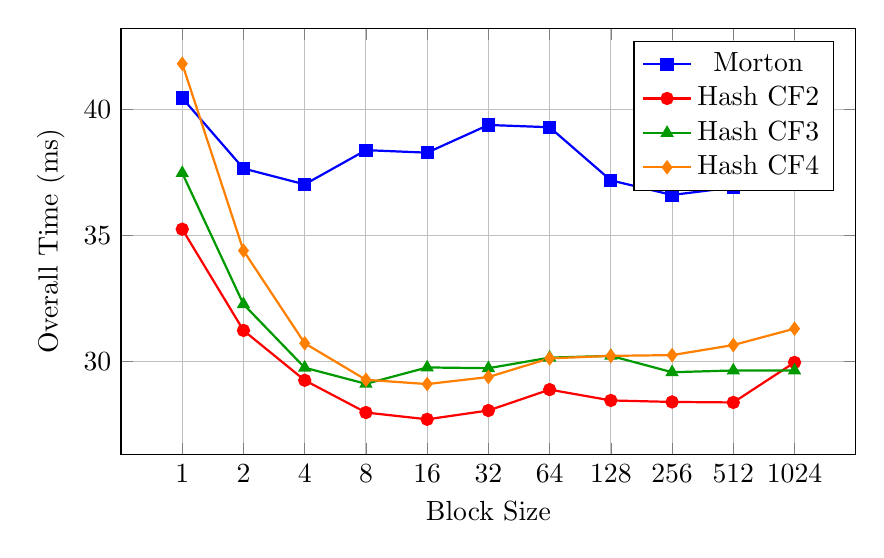
\begin{tikzpicture}
\begin{axis}[
    width=0.9\textwidth,
    height=7cm,
    xlabel={Block Size},
    ylabel={Overall Time (ms)},
    legend pos=north east,
    xmode=log,
    log basis x={2},
    xtick={1,2,4,8,16,32,64,128,256,512,1024},
    xticklabels={1,2,4,8,16,32,64,128,256,512,1024},
    grid=major,
    mark size=2pt,
]

% Morton
\addplot[color=blue,mark=square*,thick] coordinates {
    (1,40.46) (2,37.66) (4,37.03) (8,38.39) (16,38.29) 
    (32,39.39) (64,39.30) (128,37.19) (256,36.61) (512,36.91) (1024,39.67)
};

% Hash CF2
\addplot[color=red,mark=*,thick] coordinates {
    (1,35.25) (2,31.23) (4,29.25) (8,27.97) (16,27.70) 
    (32,28.05) (64,28.88) (128,28.45) (256,28.39) (512,28.37) (1024,29.96)
};

% Hash CF3
\addplot[color=green!60!black,mark=triangle*,thick] coordinates {
    (1,37.48) (2,32.27) (4,29.75) (8,29.11) (16,29.76) 
    (32,29.73) (64,30.15) (128,30.22) (256,29.57) (512,29.64) (1024,29.64)
};

% Hash CF4
\addplot[color=orange,mark=diamond*,thick] coordinates {
    (1,41.82) (2,34.40) (4,30.72) (8,29.27) (16,29.10) 
    (32,29.38) (64,30.12) (128,30.22) (256,30.25) (512,30.65) (1024,31.30)
};

\legend{Morton, Hash CF2, Hash CF3, Hash CF4}
\end{axis}
\end{tikzpicture}
\caption{Overall execution time for voxel size 0.25}
\end{figure}

% GRAPH 2: Voxel Size 0.5
\begin{figure}[H]
\centering
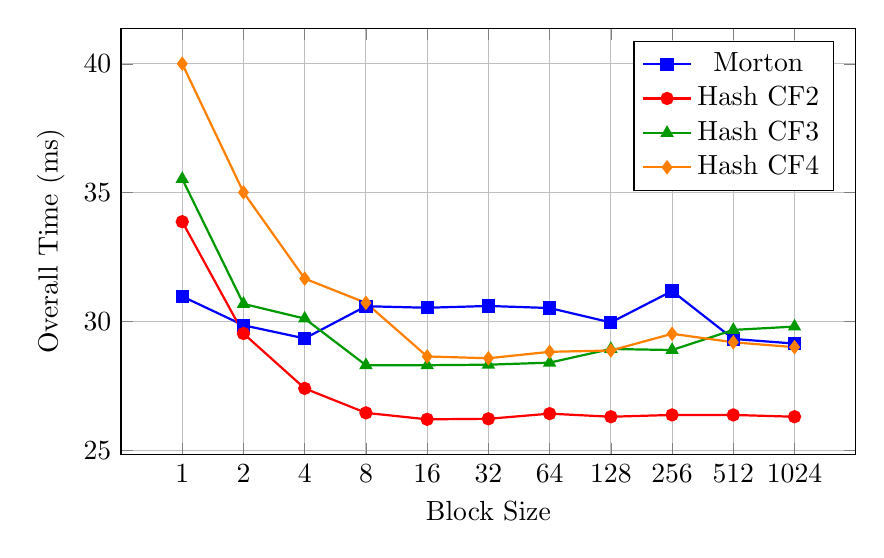
\begin{tikzpicture}
\begin{axis}[
    width=0.9\textwidth,
    height=7cm,
    xlabel={Block Size},
    ylabel={Overall Time (ms)},
    legend pos=north east,
    xmode=log,
    log basis x={2},
    xtick={1,2,4,8,16,32,64,128,256,512,1024},
    xticklabels={1,2,4,8,16,32,64,128,256,512,1024},
    grid=major,
    mark size=2pt,
]

% Morton
\addplot[color=blue,mark=square*,thick] coordinates {
    (1,30.97) (2,29.85) (4,29.34) (8,30.59) (16,30.53) 
    (32,30.60) (64,30.52) (128,29.96) (256,31.18) (512,29.32) (1024,29.14)
};

% Hash CF2
\addplot[color=red,mark=*,thick] coordinates {
    (1,33.87) (2,29.53) (4,27.40) (8,26.45) (16,26.20) 
    (32,26.22) (64,26.42) (128,26.30) (256,26.37) (512,26.37) (1024,26.30)
};

% Hash CF3
\addplot[color=green!60!black,mark=triangle*,thick] coordinates {
    (1,35.53) (2,30.68) (4,30.11) (8,28.30) (16,28.30) 
    (32,28.32) (64,28.40) (128,28.93) (256,28.89) (512,29.67) (1024,29.80)
};

% Hash CF4
\addplot[color=orange,mark=diamond*,thick] coordinates {
    (1,40.00) (2,35.01) (4,31.66) (8,30.72) (16,28.64) 
    (32,28.57) (64,28.82) (128,28.87) (256,29.52) (512,29.19) (1024,29.00)
};

\legend{Morton, Hash CF2, Hash CF3, Hash CF4}
\end{axis}
\end{tikzpicture}
\caption{Overall execution time for voxel size 0.5}
\end{figure}

% GRAPH 3: Voxel Size 0.75
\begin{figure}[H]
\centering
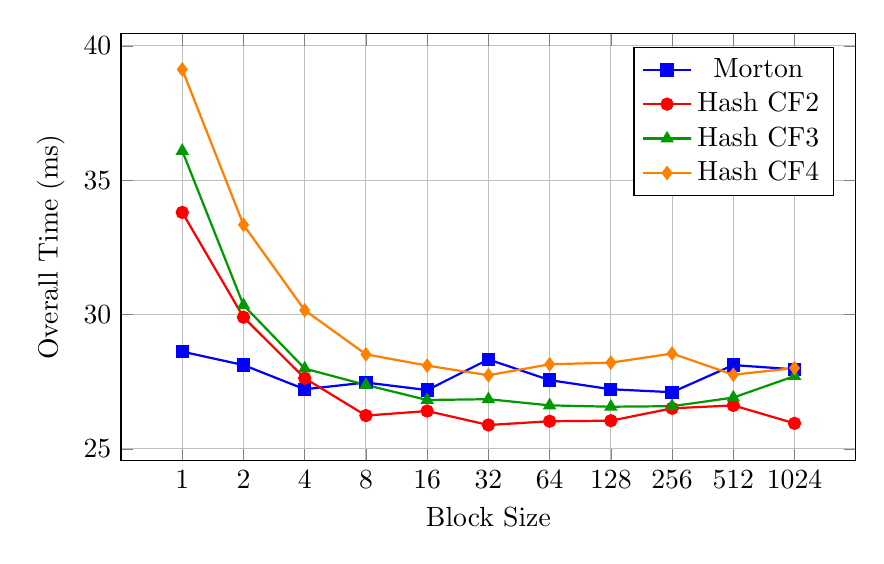
\begin{tikzpicture}
\begin{axis}[
    width=0.9\textwidth,
    height=7cm,
    xlabel={Block Size},
    ylabel={Overall Time (ms)},
    legend pos=north east,
    xmode=log,
    log basis x={2},
    xtick={1,2,4,8,16,32,64,128,256,512,1024},
    xticklabels={1,2,4,8,16,32,64,128,256,512,1024},
    grid=major,
    mark size=2pt,
]

% Morton
\addplot[color=blue,mark=square*,thick] coordinates {
    (1,28.62) (2,28.12) (4,27.22) (8,27.47) (16,27.19) 
    (32,28.33) (64,27.56) (128,27.22) (256,27.11) (512,28.12) (1024,27.96)
};

% Hash CF2
\addplot[color=red,mark=*,thick] coordinates {
    (1,33.80) (2,29.90) (4,27.63) (8,26.24) (16,26.41) 
    (32,25.89) (64,26.03) (128,26.05) (256,26.51) (512,26.62) (1024,25.95)
};

% Hash CF3
\addplot[color=green!60!black,mark=triangle*,thick] coordinates {
    (1,36.09) (2,30.35) (4,27.99) (8,27.38) (16,26.82) 
    (32,26.85) (64,26.62) (128,26.57) (256,26.59) (512,26.91) (1024,27.71)
};

% Hash CF4
\addplot[color=orange,mark=diamond*,thick] coordinates {
    (1,39.12) (2,33.34) (4,30.16) (8,28.52) (16,28.10) 
    (32,27.74) (64,28.15) (128,28.21) (256,28.55) (512,27.76) (1024,28.01)
};

\legend{Morton, Hash CF2, Hash CF3, Hash CF4}
\end{axis}
\end{tikzpicture}
\caption{Overall execution time for voxel size 0.75}
\end{figure}

% GRAPH 4: Voxel Size 1.0
\begin{figure}[H]
\centering
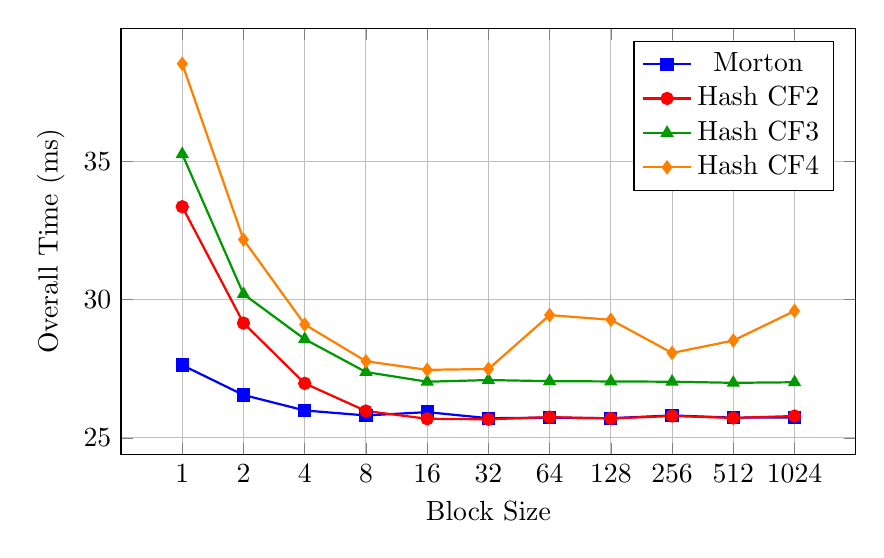
\begin{tikzpicture}
\begin{axis}[
    width=0.9\textwidth,
    height=7cm,
    xlabel={Block Size},
    ylabel={Overall Time (ms)},
    legend pos=north east,
    xmode=log,
    log basis x={2},
    xtick={1,2,4,8,16,32,64,128,256,512,1024},
    xticklabels={1,2,4,8,16,32,64,128,256,512,1024},
    grid=major,
    mark size=2pt,
]

% Morton
\addplot[color=blue,mark=square*,thick] coordinates {
    (1,27.63) (2,26.55) (4,25.99) (8,25.81) (16,25.93) 
    (32,25.71) (64,25.73) (128,25.71) (256,25.81) (512,25.73) (1024,25.74)
};

% Hash CF2
\addplot[color=red,mark=*,thick] coordinates {
    (1,33.36) (2,29.15) (4,26.97) (8,25.97) (16,25.69) 
    (32,25.67) (64,25.75) (128,25.70) (256,25.79) (512,25.72) (1024,25.79)
};

% Hash CF3
\addplot[color=green!60!black,mark=triangle*,thick] coordinates {
    (1,35.26) (2,30.20) (4,28.57) (8,27.38) (16,27.03) 
    (32,27.09) (64,27.05) (128,27.04) (256,27.03) (512,26.99) (1024,27.01)
};

% Hash CF4
\addplot[color=orange,mark=diamond*,thick] coordinates {
    (1,38.53) (2,32.17) (4,29.10) (8,27.77) (16,27.46) 
    (32,27.49) (64,29.44) (128,29.27) (256,28.07) (512,28.52) (1024,29.59)
};

\legend{Morton, Hash CF2, Hash CF3, Hash CF4}
\end{axis}
\end{tikzpicture}
\caption{Overall execution time for voxel size 1.0}
\end{figure}

% GRAPH 5: Voxel Size 1.25
\begin{figure}[H]
\centering
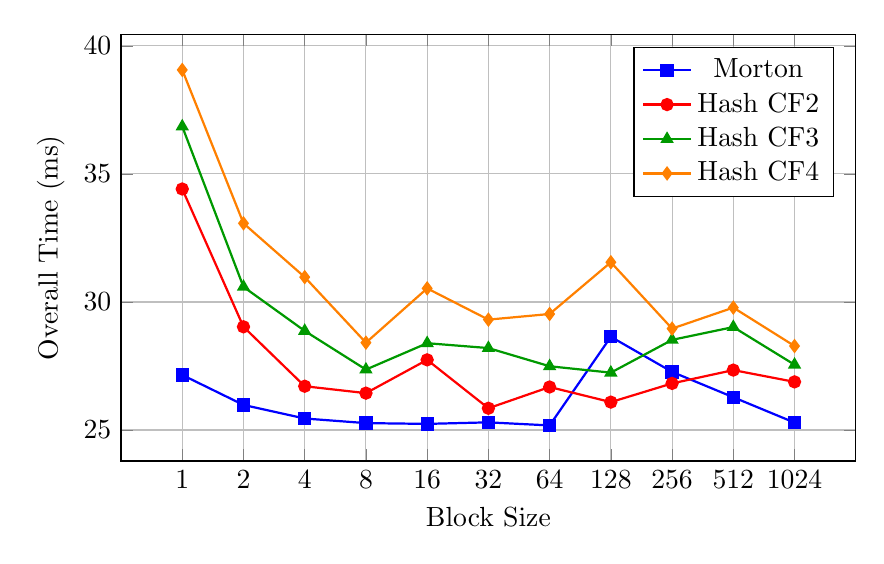
\begin{tikzpicture}
\begin{axis}[
    width=0.9\textwidth,
    height=7cm,
    xlabel={Block Size},
    ylabel={Overall Time (ms)},
    legend pos=north east,
    xmode=log,
    log basis x={2},
    xtick={1,2,4,8,16,32,64,128,256,512,1024},
    xticklabels={1,2,4,8,16,32,64,128,256,512,1024},
    grid=major,
    mark size=2pt,
]

% Morton
\addplot[color=blue,mark=square*,thick] coordinates {
    (1,27.15) (2,25.98) (4,25.45) (8,25.27) (16,25.24) 
    (32,25.30) (64,25.18) (128,28.64) (256,27.27) (512,26.28) (1024,25.29)
};

% Hash CF2
\addplot[color=red,mark=*,thick] coordinates {
    (1,34.41) (2,29.03) (4,26.71) (8,26.44) (16,27.74) 
    (32,25.85) (64,26.68) (128,26.09) (256,26.82) (512,27.34) (1024,26.88)
};

% Hash CF3
\addplot[color=green!60!black,mark=triangle*,thick] coordinates {
    (1,36.85) (2,30.59) (4,28.87) (8,27.36) (16,28.39) 
    (32,28.20) (64,27.49) (128,27.24) (256,28.52) (512,29.02) (1024,27.55)
};

% Hash CF4
\addplot[color=orange,mark=diamond*,thick] coordinates {
    (1,39.06) (2,33.07) (4,30.97) (8,28.41) (16,30.53) 
    (32,29.31) (64,29.53) (128,31.55) (256,28.96) (512,29.78) (1024,28.28)
};

\legend{Morton, Hash CF2, Hash CF3, Hash CF4}
\end{axis}
\end{tikzpicture}
\caption{Overall execution time for voxel size 1.25}
\end{figure}